 
We conducted a user study to examine the productivity of our system in constructing the digital 3D mockups from 2D layouts, and the effectiveness of our system of guiding non-expert users to fabricate the physical mockups from 2D layouts. 
%
There are two experiments in our user study.
% 
In the first experiment, participants were asked to construct the digital 3D model from the same 2D layout using our system and a commercial software STUDIO, respectively, after a brief introduction.
For each participant, 10 examples were randomly selected from the 34 2D design layouts and presented to the participant for folding using our system and Studio.
A \emph{two-alternative forced choices} design was used, with the participant asked to choose which of the two systems they prefer to use considering the operation simplicity and modeling efficiency. 
%
Furthermore, participants were asked to rate our system from one to five on the necessity of layout optimization, while five indicates it is very necessary.


%
In the second experiment, participants were separated equally into two groups, one group was asked to fold a paper sheet with the printed 2D layout into a physical carton with the guide video showing the folding sequence provided by our system. Another group was asked to make a carton without the guide video. 
Each participant was assigned with the same 2D layout (Figure~\ref{fig:automatic-more}(a)) because it is not easy to imagine its final mockup from the 2D layout at the first sight.
%
The fabrication times were recorded for two groups.
%

Based on the two experiments, our goal was to test the following hypotheses:

\begin{itemize}
	\item \textbf{Hypo1:} Our system takes less time and effort to construct a digital 3D mockup than the traditional software.
	\item \textbf{Hypo2:} Our system provides novel and practical functions to generate diverse layouts.
	\item \textbf{Hypo3:} Our system is effective for guiding non-expert users to fabricate complex cartons from 2D layouts.
\end{itemize}

\comments{
\subsection{Procedure}
We began the experiment with each participant by explaining the background and the instructions of our system and STUDIO. Ten layouts from thirty-four 2D design layouts were given to participants for folding, and at least three of them would need refinement. Participants were allowed to watch the final model of the layout to instruct construction. After operating the two systems. each participant was asked to answer a questionnaire including four(??five?? not clear how to use the question of modeling experiment) questions: which of two systems participants preferred based on the simplicity of operation. which of two systems participants preferred based on the modeling time, score one to five on the necessity of layout optimization in our system. and write down the suggestions to our system.

Foe the second experiment, we separated participants into two groups, one group would fabricate the layout as shown in Figure~\ref{fig:automatic-more}(a) with a video presenting the folding sequence, and another group would fold the layout with a figure showing the layout and its final model instead of video. The fabrication time was recorded for analysis.
}




%\subsection{Discussion}

We consider our three hypotheses in turn. 
With respect to \textbf{Hypo1}, we collect the answers of the former two questions from 30 participants, all over eighteen years of age. Both male and female participants were included, and non had experience on designing or folding cartons in computer softwares. 
%
The result is shown in Figure~\ref{fig:preference}. 
The chart shows that $93\%$ of participants prefer our system considering the operation simplicity, and $83\%$ of participants prefer our system considering the modeling time.
%
We also performed a paired-samples $t$-test at the level $\alpha = 0.05$ to compare the preference significance.
%
The test shows our system is significantly preferred by participants.
%
Most participants vote for our system mainly because it takes much less time to make a 3D model using our system. 
Take Figure~\ref{fig:result-more}(e) for example, participants usually spent much time on adjusting the folding angles of the creases, while only three clicks are required in our system.
%
On the other hand, one comment from the participants who preferred STUDIO is that the operation needed to learn in STUDIO is just selecting a folding edge and assigning angles, while our system requires them to learn more operations to construct the digital 3D model. 
%

With respect to \textbf{Hypo2}, 24 participants gave the highest score to our layout optimization function. 
%
In addition to explore the diversity of 2D layouts, it also can adjust the imprecise panels on the 2D layout to reach an ideal model. Figure~\ref{fig:correction} shows the final models constructed by our system and STUDIO, respectively. As we can see, Panel 1 is higher than Panel 2 in the digital model constructed by STUDIO, because the 2D layout is not as precise as the designer wants. 
%
In comparison, our system is able to correct these design errors by merging the 3D vertexes in different panels circled in red and optimizing the 2D layout correspondingly.

%\begin{figure}
%	\centering
%	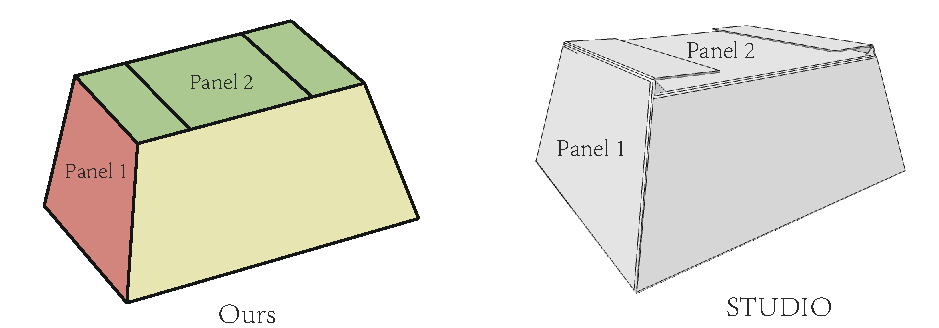
\includegraphics[width=0.5\textwidth]{images/comparison}
%	\caption{Different model constructed by our system (a) and STUDIO (b). }
%	\label{fig:correction}
%\end{figure}

Considering \textbf{Hypo3}, 38 participants (19 for each group) were asked to fabricate the 2D layout shown in Figure~\ref{fig:automatic-more}(a) into a physical carton. 
The comparison of the fabrication times with and without our guide video is shown in Figure~\ref{fig:time}. 
As we can see, most participants who did not watch the guide video spent more time, averagely 155 seconds, to folding a carton than the other group, averagely 99 seconds.
% 
%
We also performed an independent-samples $t$-test at the level $\alpha = 0.05$ to compare the fabrication time, and the result shows the guide video has significant effectiveness on the fabrication of complex cartons for non-expert users.

\begin{figure}[h]
	\centering
	\subfigure[System preference]{
		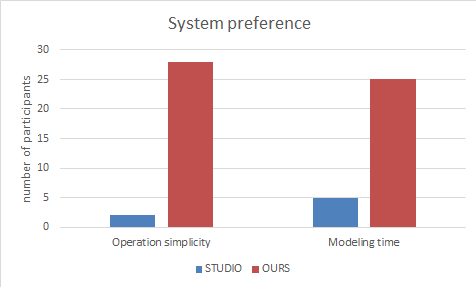
\includegraphics[width=0.25\columnwidth,height=0.11\textheight]{images/preference.png}
		\label{fig:preference}
	}
	\vspace{2ex}
	\subfigure[Layout refinment]{
		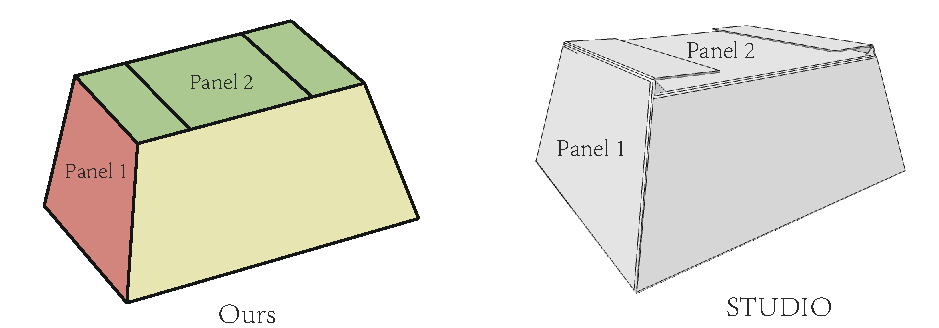
\includegraphics[width=0.35\columnwidth,height=0.08\textheight]{images/comparison}
		\label{fig:correction}
	}
	\vspace{2ex}
	\subfigure[Fabrication time]{
		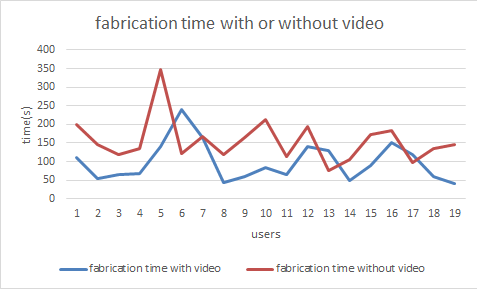
\includegraphics[width=0.25\columnwidth,height=0.11\textheight]{images/fabrication.png}
		\label{fig:time}
	}
	\caption{(a) Compared with STUDIO, more participants prefer our system considering both the operation simplicity and modeling time. (b) Our system is able to automatically refine the inaccurate 2D layout, while STUDIO only generates the folded shape based on user assigned angles. (c) Comparison of fabrication times with/without video. It took much longer time for common users to fabricate a carton from a 2D layout only without our guide process.}
	\label{fig:userstudy}
\end{figure}


